\documentclass[aspectratio=169]{beamer}
\usepackage{pgf}
\usepackage{multimedia}
\usepackage{colortbl,tabularx,mathrsfs,calligra,xcolor}
\usepackage{amsmath,amsfonts,amssymb,amsthm}
\usepackage{ragged2e}
\usepackage{setspace}
\usepackage{filecontents}
\usepackage{caption}
\usepackage{subcaption}
\usepackage{contour}
\usepackage{fancybox}
\usepackage{wrapfig}
\usepackage{multirow}
\usepackage{multicol}
\usepackage{pgfplots, tkz-euclide,calc}
    \usetikzlibrary{patterns,snakes,shapes.arrows}
\usepackage{listings}
\usepackage{enumitem}
\usepackage{pifont}
\usepackage[scaled]{berasans}
    \renewcommand*\familydefault{\sfdefault}  %% Only if the base font of the document is to be sans serif
\usepackage[T1]{fontenc}
\usepackage{hyperref}
\hypersetup{
    filecolor=magenta,      
    urlcolor=cyan,
    pdftitle={Overleaf Example},
    pdfpagemode=FullScreen,
    }
\renewcommand*\familydefault{\sfdefault} %% Only if the base font of the document is to be sans serif

\graphicspath{{C:/Users/teoso/OneDrive/Documents/Asisten Dosen & Lab/Asisten Laboratorium/Alpro 1/PPT/Graphicx/}}

\definecolor{HIMAmuda}{HTML}{01D1FD}
\definecolor{HIMAtua}{HTML}{02016A}
\definecolor{HIMAabu}{HTML}{CBCBCC}
\definecolor{PastelGreen}{HTML}{77DD77}
\definecolor{pgray}{rgb}{0.5,0.5,0.5}
\definecolor{pblue}{rgb}{0.13,0.13,1}
\definecolor{pgreen}{rgb}{0,0.5,0}
\definecolor{pred}{rgb}{0.9,0,0}
\definecolor{pgrey}{rgb}{0.46,0.45,0.48}
\definecolor{pcyan}{HTML}{D4EFFC}
\definecolor{lblue}{HTML}{00AEEF}
\definecolor{input}{HTML}{AAE1FA}
\definecolor{bg}{rgb}{0.95, 0.95, 0.92}
\definecolor{vscode}{HTML}{282A36}

\usetheme{Madrid}

\setbeamercolor{palette primary}{bg=HIMAtua,fg=white}
\setbeamercolor{palette secondary}{bg=HIMAmuda,fg=black}
\setbeamercolor{palette tertiary}{bg=HIMAabu,fg=black}
\setbeamercolor{palette quaternary}{bg=HIMAmuda,fg=white}
\setbeamercolor{structure}{fg=HIMAmuda} % itemize, enumerate, etc
\setbeamercolor{section in toc}{fg=HIMAtua} % TOC sections
\setbeamercolor{block title alerted}{fg=white,bg=magenta}
\setbeamercolor{block body alerted}{fg=black!90,bg=pink}

\usefonttheme{professionalfonts}
\setbeamertemplate{theorems}[numbered]
\setbeamertemplate{itemize items}[circle]

\usebackgroundtemplate{%
\tikz[overlay,remember picture] \node[opacity=0.1, at=(current page.center)]{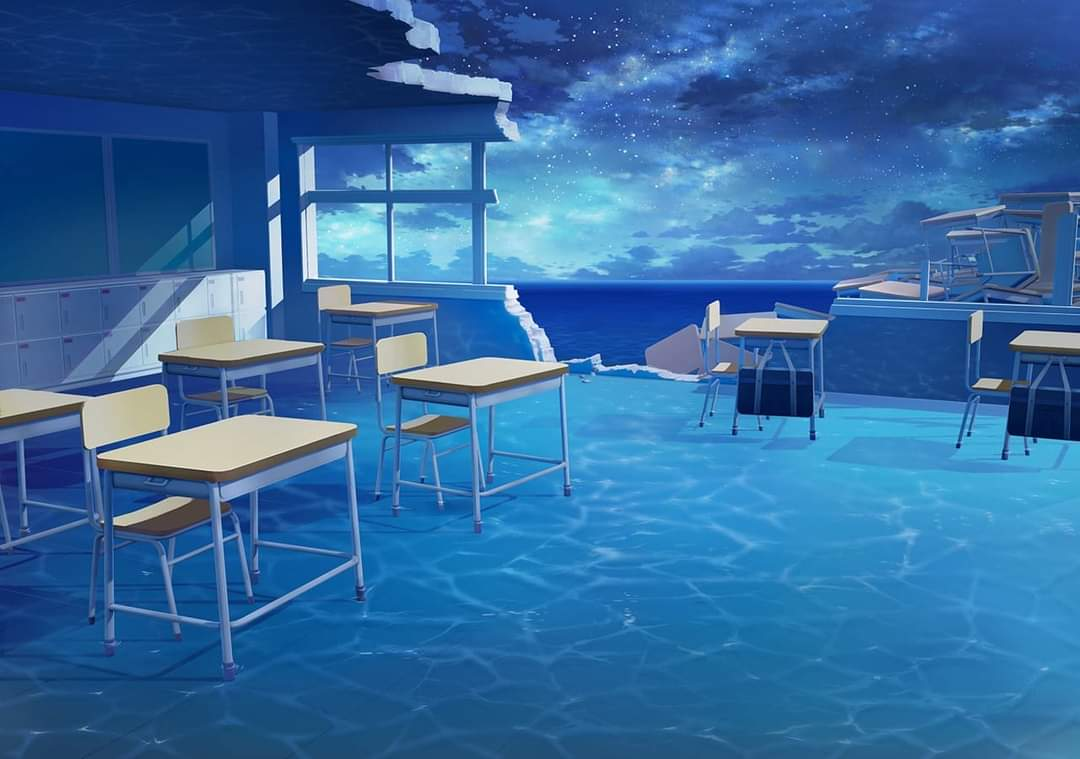
\includegraphics[width=\paperwidth]{plana class}};
}

\renewcommand\thesubfigure{\arabic{subfigure}}
\newtheorem*{funfact}{Fun Fact}
\newtheorem{latihan}{Latihan}
\newtheorem*{definisi}{Definisi}
\newtheorem{teorema}{Teorema}
\theoremstyle{definition}
\newtheorem*{contoh}{Contoh}
\newtheorem*{masalah}{Masalah}
\newcommand{\R}{\mathbb{R}}

\AtBeginEnvironment{funfact}{%
  \setbeamercolor{block title}{fg=white,bg=PastelGreen} % Set title background to pastel green and text to white
  \setbeamercolor{block body}{parent=normal text,bg=PastelGreen!30!white} % Set body background to a lighter pastel green
}
\AtBeginEnvironment{definisi}{
    \setbeamercolor{block title}{fg=white,bg=HIMAtua}
    \setbeamercolor{block body}{parent=normal text,bg=HIMAtua!30!white}
}
\AtBeginEnvironment{teorema}{
    \setbeamercolor{block title}{bg=darkgray,fg=white}
    \setbeamercolor{block body}{parent=pallette tertiary,bg=HIMAabu!30!white}
}
\AtBeginEnvironment{latihan}{%
  \setbeamercolor{block title}{fg=white,bg=PastelGreen} % Set title background to pastel green and text to white
  \setbeamercolor{block body}{parent=normal text,bg=PastelGreen!30!white} % Set body background to a lighter pastel green
}
\AtBeginEnvironment{masalah}{%
  \setbeamercolor{block title}{fg=white,bg=teal} % Set title background to pastel green and text to white
  \setbeamercolor{block body}{parent=normal text,bg=teal!30!white} % Set body background to a lighter pastel green
}

\renewcommand{\arraystretch}{1.3}

\usepackage{listings}

\lstdefinestyle{standard}{
    language            = Java,
    showspaces          = false,
    showtabs            = false,
    breaklines          = true,
    showstringspaces    = false,
    breakatwhitespace   = true,
    commentstyle        = \color{pgray},
    keywordstyle        = \color{pblue},
    stringstyle         = \color{pgreen},
    basicstyle          = \footnotesize\ttfamily,
    frame               = single,
    backgroundcolor     = \color{brown!10!white},
    escapeinside        = {(*}{*)},
    numbers             = left, % {none, left, right}
    numberstyle         = \scriptsize\color{black},
    numbersep           = -8pt,
    }

\lstdefinestyle{output}{
    language=Java,
    backgroundcolor     =\color{vscode},
    basicstyle          =\footnotesize\ttfamily\color{white},
    frame               =shadowbox,
    escapeinside        ={(*}{*)},
    showspaces          =false,
    showtabs            =false,
    breaklines          =true,
    showstringspaces    =false,
    breakatwhitespace   =true,
    rulesepcolor        =\color{HIMAtua!50!white},
    rulecolor           =\color{HIMAtua!50!white},
    numbers             =none,
    }

\lstset{style=standard}

\newcommand{\enter}{\raisebox{-1.8pt}{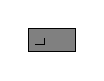
\begin{tikzpicture}[scale=0.3]
    \draw[thin,fill=gray] (0,0) rectangle (2,1);
    \draw (0.3,0.3) -- (0.7,0.3)--(0.7,0.6);     
\end{tikzpicture}}}

\newcommand{\inputscan}[1]{\raisebox{0pt}[1pt]{\colorbox{darkgray}{#1}}}

\author[Tew \& Haf]{Hafidz Mulia\\Teosofi Hidayah Agung}
\date{23 September 2024}
\title[Alpro 1 - Week 3]{Input dan Casting}
\institute[Matematika ITS]{Departemen Matematika\\ Institut Teknologi Sepuluh Nopember}
\titlegraphic{{
\includegraphics[scale=0.02]{M.png}$\quad$
\includegraphics[scale=0.2]{Provicom.png}}}

\begin{document}
    {\usebackgroundtemplate{
        \tikz[overlay,remember picture] \node[opacity=0.2, at=(current page.center)]{
\includegraphics[width=\paperwidth]{bg_2}};}
    \begin{frame}
        \titlepage
    \end{frame}
    }

    \AtBeginSection{
    {\usebackgroundtemplate{
     \tikz[overlay,remember picture] \node[opacity=0.1, at=(current page.center)]{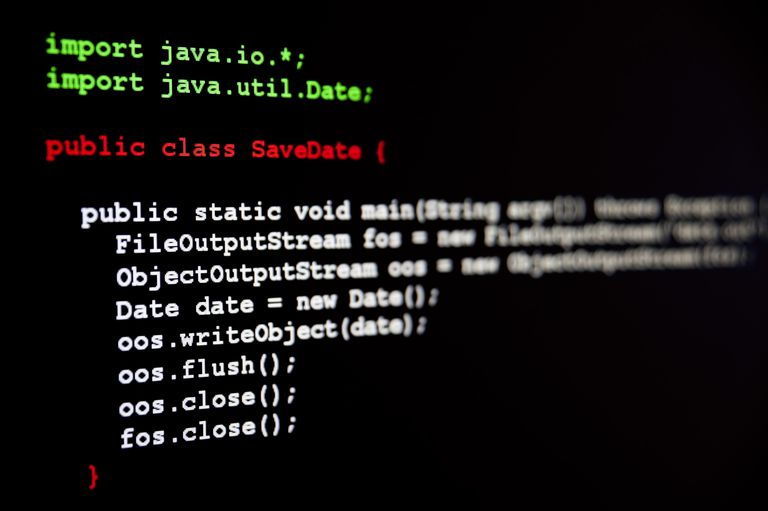
\includegraphics[width=\paperwidth]{Java code}};}
    \begin{frame}{Daftar isi}
        \tableofcontents[currentsection]
    \end{frame}}
    }

    \section{Input}
    \begin{frame}
        \frametitle{\insertsection}
        \begin{masalah}
            Bicara soal sosmed pastinya ada yang namanya username dan password. Nah, bagaimana cara kita menginputkan username dan password tersebut ke dalam program kita? Apakah kita perlu masuk ke programnya dan membuat variabelnya secara manual?
        \end{masalah}
    \end{frame}
    
    \begin{frame}
        \frametitle{\insertsection}
        \begin{definisi}
            \textbf{Input} adalah proses memasukkan data ke dalam program komputer. Data yang dimasukkan dapat berupa angka, huruf, karakter, dan lain-lain. Data yang dimasukkan dapat berasal dari keyboard, mouse, atau perangkat lainnya. Disini kita masih membatasi inputan kita dari keyboard.
        \end{definisi}
        \onslide<2->{
        \begin{block}{Scanner}
            Scanner adalah sebuah class yang ada di Java yang digunakan untuk mengambil inputan dari user. Scanner ini ada di package \texttt{java.util.Scanner} dan untuk menggunakan Scanner, kita harus mengimport package tersebut terlebih dahulu.
        \end{block}
        }
    \end{frame}

    \begin{frame}[fragile]
        \frametitle{\insertsection}
        \begin{lstlisting}[caption={Contoh penggunaan Scanner}]
    import java.util.Scanner; 
    // Import Scanner dari package java.util

    public class Input {
        public static void main(String[] args) {
            Scanner input = new Scanner(System.in); 
            // Membuat objek Scanner dengan nama "input"
            System.out.print("Masukkan nama Anda: ");
            String nama = input.nextLine(); // Mengambil inputan dari user
            System.out.println("Halo, " + nama + "!");
        }
    }
        \end{lstlisting}
    \end{frame}

    \begin{frame}[fragile]
        \frametitle{\insertsection}
        \begin{lstlisting}[style=output,title=Output \#1]
    Masukkan nama Anda: (*\inputscan{Teo}*) (*\enter*)
    Halo, Teo
        \end{lstlisting}
        \begin{lstlisting}[style=output,title=Output \#2]
    Masukkan nama Anda: (*\inputscan{Hafidz}*) (*\enter*)
    Halo, Hafidz
        \end{lstlisting}
    \vspace*{0.5cm}
    \onslide<2->{
        Bagaimana jika kita menginputkan \texttt{123} pada program tersebut? 
    }
    \end{frame}

    \begin{frame}
        \frametitle{\insertsection}
        \begin{table}
            \centering
            \begin{tabular}{|c|c|}
                \hline
                \rowcolor{HIMAmuda}  
                \textbf{Method} & \textbf{Deskripsi} \\
                \hline
                \texttt{next()} & Mengambil inputan hingga spasi \\
                \hline
                \texttt{nextLine()} & Mengambil inputan hingga baris baru \\
                \hline
                \texttt{nextInt()} & Mengambil inputan berupa integer \\
                \hline
                \texttt{nextDouble()} & Mengambil inputan berupa double \\
                \hline
                \texttt{nextBoolean()} & Mengambil inputan berupa boolean \\
                \hline
            \end{tabular}
            \caption{Method dari Scanner}
        \end{table}
        \vspace*{0.5cm}
        Sesuaikan method yang digunakan dengan tipe data yang ingin diinputkan.
    \end{frame}

    \section{Casting}
    \begin{frame}
        \frametitle{\insertsection}
        \begin{masalah}
            Bermula ketika kita ingin membagi \texttt{int} dengan \texttt{int}. Hasil yang inginkan sebenarnya adalah bilangan desimal, namun hasil yang dikeluarkan adalah pembulatan ke bawah dari hasil sebenarnya. Bagaimana cara kita mengubah hasil tersebut menjadi bilangan desimal?
        \end{masalah}
        \onslide<2->{
        \begin{definisi}
            \textbf{Casting} adalah proses mengubah tipe data dari suatu variabel ke tipe data lain. Casting dilakukan ketika kita ingin mengubah tipe data dari variabel yang sudah ada ke tipe data yang lain.
        \end{definisi}
        }
    \end{frame}

    \begin{frame}
        \frametitle{\insertsection}
        \begin{columns}
            \begin{column}{0.45\textwidth}
                \begin{block}{Widening Casting}
                    Wide artinya lebar, jadi Widening Casting adalah proses casting dari tipe data yang lebih sempit ke tipe data yang lebih lebar. Pada dasarnya kita hanya mengubah deklarasi variabelnya saja.
                \end{block}
            \end{column}
            \begin{column}{0.45\textwidth}
                \begin{block}{Narrowing Casting}
                    Narrow artinya sempit, jadi Narrowing Casting adalah proses casting dari tipe data yang lebih lebar ke tipe data yang lebih sempit. Pada proses ini kita harus menggunakan tanda kurung sebelum variabel yang akan di-casting.
                \end{block}
            \end{column}
        \end{columns}
        \vspace*{0.5cm}
        Berdasarkan besarnya ukuran tipe data bisa dilihat dari hubungan berikut:
        \[\texttt{byte} < \texttt{short} < \texttt{int} < \texttt{long} < \texttt{float} < \texttt{double}\]
    \end{frame}

    \begin{frame}[fragile]
        \frametitle{\insertsection}
        \begin{lstlisting}[caption={Contoh penggunaan Casting}]
    public class Casting {
        public static void main(String[] args) {
            int x = 10;
            double y = x; // Widening Casting
            System.out.println("Nilai x: " + x);
            System.out.println("Nilai y: " + y);
            System.out.println();

            double z = 20.5;
            int w = (int) z; // Narrowing Casting
            System.out.println("Nilai z: " + z);
            System.out.println("Nilai w: " + w);
        }
    }
        \end{lstlisting}
    \end{frame}

    \begin{frame}[fragile]
        \begin{exampleblock}{Contoh}
            Telusuri dan simpulkan output dari program berikut!
        \end{exampleblock}
        \begin{lstlisting}
    public class Latihan {
        public static void main(String[] args) {
            int a = 2, b = 5;
            double c = 0.5;
            System.out.println("a + b = " + a + b);
            System.out.println("a + c = " + a + c);
            System.out.println("b / c = " + b / c);
            System.out.println("b / c = " + (int)(b / c));
            System.out.println("a / b = " + a / b);
            System.out.println("a / b = " + (double)a / b);
        }
    }
        \end{lstlisting}
    \end{frame}

    {
    \setbeamercolor{block title}{bg=darkgray,fg=white}
    \setbeamercolor{block body}{parent=pallette tertiary,bg=HIMAabu!30!white}
    \begin{frame}
        \begin{alertblock}{Perhatikan}
            Selanjutnya akan diajarkan tentang manipulasi angka desimal. Namun cara dibawah ini hanyalah salah satu cara, masih banyak cara lain yang bisa digunakan tergantung prefensi masing-masing orang.
        \end{alertblock}
        \onslide<2->{
        \begin{block}{Manipulasi Angka Desimal}
            \begin{itemize}[label=$\Rightarrow$]
                \item Dimulai dari sebuah variabel bertipe \texttt{double} atau \texttt{float}.
                \item Variabel tersebut kalikan dengan $10^n$ dimana $n$ adalah jumlah angka di belakang koma yang diinginkan.
                \item Casting variabel tersebut menjadi \texttt{int}.
                \item Bagi variabel tersebut dengan $10^n$ bertipe double dengan cara tambahkan \texttt{.0} dibelakang angkanya. 
            \end{itemize}
        \end{block}}
    \end{frame}
    }

    \begin{frame}[fragile]
        \begin{exampleblock}{Contoh}
            Ubahlah angka desimal 3.14159 menjadi 3.14
        \end{exampleblock}
        \begin{lstlisting}[caption={Manipulasi Angka Desimal}]
    double pi = 3.14159;
    int pi2 = (int)(pi * 100);
    double pi3 = pi2 / 100.0;
    System.out.println(pi3);            
        \end{lstlisting}
    \end{frame}

    \section{Latihan}
    \begin{frame}
        \begin{latihan}
            Buatlah program yang meminta inputan jari-jari lingkaran dan menghitung luas lingkaran tersebut. (Cukup 2 angka di belakang koma)\\

            \textbf{Hint:} Gunakan \texttt{Math.PI} untuk mengakses nilai $\pi$.
        \end{latihan}
        \begin{latihan}
            Disebuah perusahaan, gaji karyawan dihitung berdasarkan jam kerja yaitu Rp50.000,- per jam. Kemudian juga terdapat potongan pajak sebesar $\displaystyle\frac{3}{35}$ dari gaji karyawan. Buatlah program yang meminta inputan jam kerja karyawan dan menghitung gaji bersih karyawan tersebut dalam rupiah.
        \end{latihan}
    \end{frame}
\end{document}